\documentclass[11pt]{article}
% Suggested arXiv categories: cs.AI (primary), cs.GT (secondary)

% Encoding & typography
\usepackage[T1]{fontenc}
\usepackage[utf8]{inputenc}
\usepackage{lmodern}
\usepackage[margin=1in]{geometry}
\usepackage{microtype}

% Math / tables / figures
\usepackage{amsmath,amssymb}
\usepackage{booktabs}
\usepackage{graphicx}
\usepackage{caption}

% Links / lists / authors
\usepackage[hidelinks]{hyperref}
\usepackage{enumitem}
\usepackage{authblk}
\usepackage{tikz}
\usepackage{pgfplots}
\pgfplotsset{compat=1.18}
\usepackage{fancyvrb}
\usepackage[table]{xcolor}

\newcommand{\tOne}{T001}
\newcommand{\tTwo}{T002}
\newcommand{\tThree}{T003}

\title{Moreau Arena: Not All LLMs Need Hints to Reason Strategically}

\author[1]{Victor Stasiuc}
\affil[1]{Independent Researcher\\
\texttt{stvitek@gmail.com}\\
ORCID: \href{https://orcid.org/0009-0003-2064-0486}{0009-0003-2064-0486}}

\date{March 2026}

\begin{document}
\maketitle

\vspace{-0.7em}
\begin{abstract}
We introduce Moreau Arena, a contamination-resistant benchmark for LLM strategic reasoning.
Agents design creature builds (animal choice plus stat allocation) for a novel stochastic combat game whose rules exist only in the prompt.
Three tournaments over the same benchmark core---13 agents in \tOne/\tTwo, expanded to 15 in \tThree---and 2609 best-of-7 series reveal a sharp boundary condition.
Under vague rules with no feedback (\tOne), baselines dominate and LLMs win only 37.5\% of cross-group series.
With exact formulas, meta-context hints, and per-game adaptation (\tTwo), the leaderboard reverses: LLMs win 89.75\%.
A targeted ablation (\tThree) removes only the meta-context hints while preserving exact rules and feedback.
Performance does not collapse uniformly; instead the field splits.
GPT-5.2-Codex and Claude~Opus remain strong without hints, while three models from three providers freeze on a single identical build and never adapt.
Meanwhile, GPT-5.4---released during this study---ranks 14th of 15 despite exploring 79~builds, demonstrating that frontier capability does not automatically transfer to novel strategic domains.
A prompt sensitivity analysis using semantically equivalent paraphrases of the \tThree{} prompt yields Kendall $\tau=1.0$ (perfect rank preservation), confirming that the key findings are not prompt-dependent artifacts.
We release all prompts, match records, configuration hashes, and analysis code at \url{https://moreauarena.com}.
\end{abstract}

\section{Introduction}

Large language models (LLMs) increasingly act as decision-makers in interactive settings: recommending actions, planning under uncertainty, and adapting to opponents.
Yet evaluating strategic reasoning is difficult: many benchmarks are either too static (single-step questions) or too contaminated (popular games and well-known strategies).

We introduce \textbf{Moreau Arena}, a compact, synthetic strategy benchmark designed to stress quantitative trade-offs while minimizing training-data leakage.
An agent chooses one of six animals offered in the prompt (bear, buffalo, boar, monkey, tiger, wolf) and allocates 20 stat points across health (HP), attack (ATK), speed (SPD), and willpower (WIL).
The game then simulates stochastic combat under fixed rules.
(The underlying simulator supports additional species for internal testing; one baseline, RandomAgent, samples from the full roster and happens to select \texttt{raven} under its fixed seed.)

This paper reports a controlled comparison of \textbf{three tournaments built on the same core environment}.
The core question is not ``can LLMs play the game'' but \emph{what conditions let LLMs express strategic competence}.
Tournament~001 (\tOne) is intentionally under-specified (qualitative abilities; no feedback), exposing systematic failure modes.
Tournament~002 (\tTwo) removes confounds by providing exact numerical formulas, injecting meta knowledge, requiring structured outputs, and enabling per-game adaptation.
Tournament~003 (\tThree) is a targeted ablation that preserves exact rules and feedback while removing only the meta-context block, thereby isolating the role of explicit meta initialization.

\subsection*{Contributions}

This paper contributes:
\begin{enumerate}[leftmargin=*]
\item A newly authored game environment (Moreau Arena) designed to reduce contamination risk and to admit a derivable dominant strategy under a frozen configuration snapshot.
\item Two 13-agent round-robin tournaments (8 frontier LLMs, 5 baselines), totaling 1559 best-of-7 series under different information scaffolding regimes.
\item A third no-meta ablation tournament (\tThree) with 15~agents and 1050~series, revealing that some models remain strategically robust without hints while others collapse to rigid default builds.
\item A negative-transfer result: GPT-5.4, a state-of-the-art frontier model, ranks 14th of 15 despite active exploration, showing that general capability does not imply strategic competence in novel domains.
\item A prompt sensitivity validation (Kendall $\tau=1.0$ under a semantically equivalent paraphrase) confirming that \tThree{} findings are not prompt-dependent artifacts.
\item Evidence that the \tOne$\to$\tTwo performance reversal implicates comprehension and feedback rather than an absence of strategic capability, with model-specific meta-initialization dependence as the key moderator.
\end{enumerate}

\section{Related Work}

\paragraph{Strategic agents and games.}
CICERO~\cite{cicero} combines language models with planning to achieve strong play in Diplomacy, while Pluribus~\cite{pluribus} demonstrates superhuman play in multiplayer poker.
Such games are strategically rich, but they are heavily documented, increasing the likelihood that modern LLMs have seen strategies or transcripts during training.

\paragraph{Game-based benchmarks.}
Orak~\cite{orak} evaluates LLM agents across 12 real video games and was presented at ICLR 2026.
While Orak provides ecological validity through familiar games, it inherits visual parsing overhead, legacy mechanics, and uncontrollable game complexity.
Moreau Arena complements Orak by isolating \emph{pure strategic reasoning}: all state is textual, combat is deterministic given a seed, and the game mechanics are novel.
The NetHack Learning Environment (NLE)~\cite{nle} and procedurally generated RL benchmarks~\cite{procgen} aim to measure generalization in challenging domains.
These environments are not primarily designed to test whether a model can derive an optimal strategy from a compact rulesheet without interaction or learning.

\paragraph{In-context learning and prompt sensitivity.}
Recent work has shown that LLM performance on reasoning tasks is highly sensitive to prompt framing.
Min et al.~\cite{min2022} find that in-context examples improve performance even when labels are randomized, suggesting that format priming matters as much as content.
Wei et al.~\cite{wei2022} demonstrate that chain-of-thought prompting can unlock reasoning capabilities otherwise absent under direct prompting.
Our three-tournament design directly probes this phenomenon: the same models under different information scaffolding show dramatically different strategic performance, and \tThree{} isolates which component of that scaffolding each model depends on.

\paragraph{Reasoning benchmarks.}
Widely used datasets such as MMLU~\cite{mmlu}, GSM8K~\cite{gsm8k}, BIG-bench~\cite{bigbench}, and ARC~\cite{arc} test isolated reasoning skills, often in non-adversarial settings.
They do not directly measure one-shot \emph{strategic} reasoning where a single decision must integrate multiple mechanics under competition.

\paragraph{Evaluation methodology.}
Preference-based leaderboards such as LMSYS Chatbot Arena~\cite{chatbot_arena} and broad evaluation suites such as HELM~\cite{helm} provide useful comparative signals but depend on human judgments and may conflate helpfulness with capability.
Moreau Arena uses objective win/loss outcomes from a seeded simulator and paired-comparison modeling.
We adopt Bradley--Terry ranking~\cite{bradley_terry}, widely used for paired outcomes, as our primary metric and include Elo only as a secondary, path-dependent score.

\section{Moreau Arena}

\paragraph{Game core.}
Each agent selects (i) one animal from the prompt roster and (ii) a stat allocation with HP+ATK+SPD+WIL=20 (each $\ge 1$).
Animals provide passives and a low-probability special ability; outcomes are stochastic due to random ability procs and tie-break rules.
A ``series'' is first-to-4 wins (best-of-7 in decisive games), but drawn games can occur and do not increment the score, so the number of simulated games per series can exceed~7.
Matches take place on an 8$\times$8 grid for at most 60 ticks; a closing ring begins at tick~30 and damages creatures on outer tiles, shrinking the safe zone to 4$\times$4 by tick~40.

\paragraph{Why ATK stacking is a derivable dominant strategy.}
The stat formulas are:
\[
\texttt{max\_hp} = 50 + 10\cdot \texttt{HP},\qquad
\texttt{base\_dmg} = \left\lfloor 2 + 0.85\cdot \texttt{ATK}\right\rfloor,
\]
\[
\texttt{dodge} = \min(30\%, 2.5\%\cdot \texttt{SPD}),\qquad
\texttt{resist} = \min(60\%, 3.3\%\cdot \texttt{WIL}).
\]
ATK=14 yields base\_dmg=13, while ATK=8 yields 8---a 62.5\% increase for 6 points.
By comparison, 6 points of HP add only 60 max HP, often insufficient to offset faster time-to-kill under ring pressure.
Proc rates (3.5--4.5\% per tick) are low enough that proc-focused or resistance-focused allocations have small expected value.

\paragraph{Contamination resistance.}
The animals, abilities, and numerical parameters are bespoke to this benchmark.
Agents cannot rely on memorized openings or known metas; they must infer trade-offs from the prompt (\tOne) or apply explicit mechanics (\tTwo, \tThree).

\paragraph{Auto-balancer (benchmark as a living test).}
A common failure mode in synthetic strategy benchmarks is ``overfitting the ruleset'': once a single dominant build is found, the benchmark collapses into a static lookup task.
Moreau Arena includes an \emph{auto-balancer} that can be enabled between tournaments to keep the meta non-stationary.
After each tournament, each animal's empirical win rate is tracked with an exponential moving average (EMA) with smoothing $\alpha=0.15$.
Proc probabilities are then nudged by a small multiplicative adjustment with coefficient $\beta=0.03$ in the direction that reduces deviation from a target 50\% win rate, with clipping to keep parameters in a valid range:
\[
\mathrm{EMA}_{t+1} = \alpha w_t + (1-\alpha)\mathrm{EMA}_t,\qquad
p_{t+1} = \mathrm{clip}\!\left(p_t\left(1+\beta(0.5-\mathrm{EMA}_t)\right)\right).
\]
This makes the benchmark a repeated-game setting rather than a one-and-done puzzle.
\textbf{In this paper, the auto-balancer is disabled and the game configuration is frozen across \tOne, \tTwo, and \tThree} to isolate prompting and feedback effects.

\section{Experimental Setup}
\label{sec:setup}

\subsection{Agents}

We evaluate 13 agents in \tOne{} and \tTwo: eight frontier LLMs and five non-LLM baselines.
Tournament~003 adds two exploratory challengers (\texttt{gpt-5.3-codex} and \texttt{gpt-5.4}) for a total of 15 agents.

\paragraph{LLMs.}
Claude Opus 4.6, Claude Sonnet 4.6, Claude Haiku 4.5 (Anthropic);
GPT-5.2 and GPT-5.2 Codex (OpenAI);
Gemini 3 Flash and Gemini 3.1 Pro (Google);
Grok 4.1 Fast (xAI).
Tournament~003 additionally includes \texttt{gpt-5.3-codex} and \texttt{gpt-5.4}.

\paragraph{Baselines.}
\emph{SmartAgent} performs internal simulation (200 match rollouts) over a candidate build set and selects the empirically best build; in \tTwo{} and \tThree{} it re-evaluates candidates after observing the winner's build, producing up to 5 distinct builds across its series.
\emph{HighVarianceAgent} hard-codes the glass-cannon build \texttt{bear 3/14/2/1}.
\emph{ConservativeAgent} hard-codes a high-HP buffalo build (\texttt{buffalo 8/6/4/2}).
\emph{GreedyAgent} uses a hand-written lookup policy (\texttt{boar 8/8/3/1}).
\emph{RandomAgent} samples from the full simulator roster under a fixed seed, producing \texttt{raven 3/3/2/12} deterministically; it serves as a floor baseline.

\subsection{Tournament protocols}

Both \tOne{} and \tTwo{} use the same round-robin schedule over all $\binom{13}{2}=78$ pairings, with 10 independent series per pairing (780 planned series).
Tournament~003 uses the same protocol family but over 15 agents, giving $\binom{15}{2}=105$ pairings and 1050 series.

\paragraph{Tournament 001 (\tOne): one-shot blind pick.}
Agents receive qualitative descriptions of animals and abilities (Appendix~\ref{app:t1_prompt}) and output a single build per series.
Agents do not observe opponent choices or results during build selection.
\tOne{} contains 779 completed series due to one runtime error in a single pairing.

\paragraph{Tournament 002 (\tTwo): exact formulas + meta + per-game adaptation.}
\tTwo{} adds four major interventions simultaneously:
(1) exact numerical formulas for damage, procs, and ring mechanics;
(2) meta context in the prompt (top-performing builds automatically extracted from \tOne{} match records; see Appendix~\ref{app:t2_prompt} for the exact injected text);
(3) structured JSON output constrained by a per-provider schema;
(4) per-game adaptation within each series---after each game, the loser sees the winner's build and may re-pick, while the winner's build is locked.

Meta context was extracted automatically by filtering out floor baselines (RandomAgent, HighVarianceAgent) and ranking remaining builds by win rate on the filtered subset.
All five injected builds showed 100\% win rate on their respective subsamples (4--22 games each), though game-level win rates across all agents are lower (80--100\%; see Appendix~\ref{app:t2_prompt}).

\paragraph{Tournament 003 (\tThree): exact formulas + feedback, no meta.}
\tThree{} is a targeted ablation of \tTwo{}.
It preserves exact formulas, structured outputs, and loser adaptation, but removes the meta-context block entirely.
Thus, \tThree{} isolates the role of explicit meta initialization while leaving the rest of the \tTwo{} scaffolding intact.
Prompt verification confirms that no build hints or meta-performance summaries were present in the \tThree{} prompts.

\begin{table}[h]
\centering
\small
\caption{Summary of protocol differences between tournaments.}
\label{tab:protocol}
\begin{tabular}{p{0.28\columnwidth} p{0.28\columnwidth} p{0.28\columnwidth}}
\toprule
Tournament~001 & Tournament~002 & Tournament~003 \\
\midrule
One-shot per series & Per-game adaptation (loser repicks; winner locked) & Per-game adaptation (loser repicks; winner locked) \\
Blind pick & Loser sees opponent animal+stats & Loser sees opponent animal+stats \\
Qualitative ability text & Exact numerical formulas & Exact numerical formulas \\
No meta context & Top-5 builds injected from \tOne & No meta context \\
Free-text output & Strict JSON schema per provider & Strict JSON schema per provider \\
\bottomrule
\end{tabular}
\end{table}

\subsection{Metrics}

We report:
(i) Bradley--Terry (BT) scores fit to pairwise series outcomes, normalized to $[0,1]$ with 95\% bootstrap confidence intervals;
(ii) Elo ratings computed over series outcomes as an auxiliary perspective;
(iii) series win--loss totals from the round-robin;
(iv) build diversity (unique builds used) and adaptation metrics in \tTwo{} and \tThree.

\section{Tournament 001 Results: One-Shot Strategy Failure}

\subsection{Baselines dominate}

Table~\ref{tab:t1_rank} and Figure~\ref{fig:t1_bt} summarize \tOne.
The top three ranks are occupied by non-LLM baselines (SmartAgent, HighVarianceAgent, ConservativeAgent), while the best LLM (Gemini Flash) ranks 4th with BT=0.503.
LLMs win only 150/400=37.50\% of LLM-vs-baseline series.

\begin{table}[t]
\centering
\small
\caption{Tournament~001 rankings by Bradley--Terry (BT) score with 95\% bootstrap confidence intervals, plus Elo and series records.}
\label{tab:t1_rank}
\begin{tabular}{rllclrr}
\toprule
Rank & Agent & Type & BT (95\% CI) & Elo & W--L & Ser. \\
\midrule
1 & SmartAgent & Base & 1.000 [.610, 1.000] & 1672 & 99--21 & 120 \\
2 & HighVariance & Base & 0.954 [.555, 1.000] & 1632 & 98--22 & 120 \\
3 & Conservative & Base & 0.643 [.372, .917] & 1780 & 89--31 & 120 \\
4 & Gemini Flash & LLM & 0.503 [.267, .771] & 1718 & 83--37 & 120 \\
5 & Gemini Pro & LLM & 0.455 [.247, .678] & 1682 & 80--39 & 119 \\
6 & Grok-4.1 Fast & LLM & 0.437 [.230, .665] & 1865 & 79--40 & 119 \\
7 & Greedy & Base & 0.239 [.128, .346] & 1362 & 64--56 & 120 \\
8 & GPT-5.2 & LLM & 0.230 [.122, .343] & 1439 & 63--57 & 120 \\
9 & GPT-5.2-Codex & LLM & 0.119 [.067, .168] & 1477 & 47--73 & 120 \\
10 & Cl.\ Sonnet 4.6 & LLM & 0.066 [.034, .097] & 1528 & 34--86 & 120 \\
11 & Cl.\ Haiku 4.5 & LLM & 0.056 [.030, .081] & 1396 & 31--89 & 120 \\
12 & Cl.\ Opus 4.6 & LLM & 0.017 [.009, .024] & 1194 & 12--108 & 120 \\
13 & Random & Base & 0.005 [.003, .008] & 757 & 0--120 & 120 \\
\bottomrule
\end{tabular}
\end{table}

\begin{figure}[t]
\centering
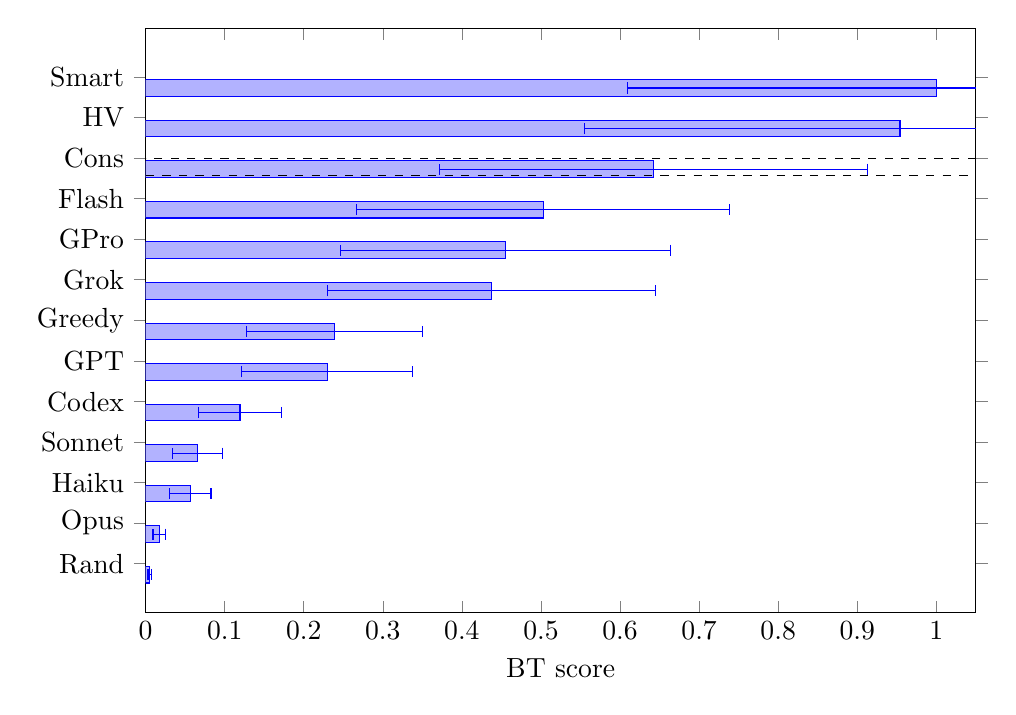
\begin{tikzpicture}
\begin{axis}[
xbar,
xmin=0, xmax=1.05,
height=9cm,
width=\columnwidth,
xlabel={BT score},
ytick={0,1,2,3,4,5,6,7,8,9,10,11,12},
yticklabels={Smart,HV,Cons,Flash,GPro,Grok,Greedy,GPT,Codex,Sonnet,Haiku,Opus,Rand},
y dir=reverse,
bar width=6pt,
error bars/x dir=both, error bars/x explicit,
]
\addplot+[error bars/x dir=both, error bars/x explicit] coordinates {
(1.0000,0) +- (0.3900,0.0000)
(0.9541,1) +- (0.3995,0.0459)
(0.6426,2) +- (0.2708,0.2744)
(0.5028,3) +- (0.2359,0.2686)
(0.4553,4) +- (0.2088,0.2229)
(0.4373,5) +- (0.2075,0.2272)
(0.2388,6) +- (0.1111,0.1068)
(0.2296,7) +- (0.1079,0.1129)
(0.1193,8) +- (0.0528,0.0482)
(0.0656,9) +- (0.0320,0.0317)
(0.0564,10) +- (0.0263,0.0241)
(0.0173,11) +- (0.0079,0.0069)
(0.0054,12) +- (0.0024,0.0024)
};
\addplot[black,dashed] coordinates {(0,2.5) (1.05,2.5)};
\end{axis}
\end{tikzpicture}
\caption{Tournament~001 BT scores with 95\% bootstrap CI. Dashed line marks the boundary below the top-3 baselines.}
\label{fig:t1_bt}
\end{figure}

\subsection{Pairwise structure}

The pairwise matrix (Table~\ref{tab:t1_matrix}) shows a largely transitive hierarchy: we find 0 strict 3-cycles where $A$ beats $B$, $B$ beats $C$, and $C$ beats $A$ (all edges $>$50\%).

\subsection{The WIL trap}

The most consistent and costly failure mode is over-investing in WIL.
Claude Opus is the extreme case: it repeats \texttt{wolf 3/8/1/8} in 85.8\% of series and averages WIL$\approx$7.9.
The \tOne{} prompt describes resistance as $\texttt{resist}=\min(60\%,3.3\%\cdot\texttt{WIL})$, which can appear large in isolation.
However, under the simulator mechanics, resist applies only to ability procs, whose base probability is 3.5--4.5\% per tick.
Even under a generous upper bound (4.5\% base proc rate), at WIL=8 the expected number of resisted procs over a 60-tick match is
\[
60 \times 0.045 \times 0.264 \approx 0.71,
\]
i.e., fewer than one blocked proc per match.
This is typically not worth sacrificing multiple points of ATK (large, reliable damage) or SPD (initiative and dodge).
Across the 8 LLMs, mean WIL is strongly negatively correlated with BT (Spearman $\rho=-0.93$, $p<0.001$), consistent with WIL acting as a systematic trap rather than a nuanced trade-off.

\subsection{Build patterns and diversity}

Table~\ref{tab:t1_build} summarizes build choices in \tOne.
Baselines are effectively fixed-build agents (unique builds$\le$2), while LLMs vary widely in exploration.
Among LLMs, build diversity correlates strongly with performance (Spearman $\rho=0.81$, $p=0.015$), suggesting that searching the build space from vague rules is a key bottleneck.

\subsection{The price paradox}

Claude models are the weakest LLM family in \tOne.
Opus is worst overall among LLMs (BT=0.017) despite being the most expensive Claude tier, while Sonnet is the strongest Claude in this tournament (BT=0.066).
The price ordering across Claude tiers (Opus $>$ Sonnet $>$ Haiku) does not predict performance ordering, suggesting that helpfulness-oriented tuning and stylistic polish do not imply stronger quantitative strategy derivation under one-shot constraints.

\begin{table}[t]
\centering
\footnotesize
\caption{Tournament~001 build patterns. ``Unique builds'' counts distinct (animal, HP, ATK, SPD, WIL) tuples across all series.}
\label{tab:t1_build}
\begin{tabular}{llcrrl}
\toprule
Agent & Top animal & Avg stats & UA & UB & Signature \\
\midrule
SmartAgent & Bear 100\% & 3/14/2/1 & 1 & 1 & bear 3/14/2/1 \\
HighVar & Bear 100\% & 3/14/2/1 & 1 & 1 & bear 3/14/2/1 \\
Conserv & Buffalo 100\% & 8/6/4/2 & 1 & 1 & buffalo 8/6/4/2 \\
Flash & Tiger 51\% & 6.4/8.8/3.6/1.2 & 4 & 53 & bear 8/10/1/1 (13\%) \\
GPro & Tiger 73\% & 6.6/8.6/3.6/1.2 & 3 & 21 & tiger 6/8/5/1 (16\%) \\
Grok & Bear 42\% & 6.2/8.1/4.3/1.4 & 6 & 60 & bear 8/8/3/1 (19\%) \\
Greedy & Boar 100\% & 8/8/3/1 & 1 & 1 & boar 8/8/3/1 \\
GPT & Tiger 61\% & 7.3/7.0/3.8/1.9 & 2 & 19 & tiger 6/8/5/1 (38\%) \\
Codex & Tiger 87\% & 5.9/7.2/5.1/1.8 & 4 & 37 & tiger 6/7/5/2 (29\%) \\
Sonnet & Wolf 99\% & 4/8/5.2/2.7 & 2 & 3 & wolf 4/8/5/3 (73\%) \\
Haiku & Tiger 68\% & 5.3/7.3/5/2.4 & 2 & 9 & tiger 4/7/6/3 (54\%) \\
Opus & Wolf 100\% & 3/8.1/1/7.9 & 1 & 2 & wolf 3/8/1/8 (86\%) \\
Random & Raven 100\% & 3/3/2/12 & 1 & 1 & raven 3/3/2/12 \\
\bottomrule
\end{tabular}
\vspace{0.3em}
\noindent\footnotesize{UA = unique animals; UB = unique builds.}
\end{table}

\begin{table}[t]
\centering
\footnotesize
\setlength{\tabcolsep}{2.5pt}
\renewcommand{\arraystretch}{1.05}
\caption{Tournament~001 pairwise series win rates (\%). Most matchups use 10 series; Gemini~Pro vs Grok uses 9 due to one runtime error.}
\label{tab:t1_matrix}
\begin{tabular}{lrrrrrrrrrrrrr}
\toprule
 & Sm & HV & Co & Fl & GP & Gr & Gy & G5 & Cx & So & Ha & Op & Ra \\
\midrule
Sm & -- & 60 & 100 & 70 & 60 & 60 & 70 & 70 & 100 & 100 & 100 & 100 & 100 \\
HV & 40 & -- & 100 & 50 & 70 & 60 & 90 & 70 & 100 & 100 & 100 & 100 & 100 \\
Co & 0 & 0 & -- & 60 & 60 & 80 & 100 & 90 & 100 & 100 & 100 & 100 & 100 \\
Fl & 30 & 50 & 40 & -- & 50 & 50 & 80 & 80 & 80 & 90 & 80 & 100 & 100 \\
GP & 40 & 30 & 40 & 50 & -- & 22 & 60 & 70 & 90 & 100 & 100 & 100 & 100 \\
Gr & 40 & 40 & 20 & 50 & 78 & -- & 70 & 80 & 70 & 50 & 100 & 100 & 100 \\
Gy & 30 & 10 & 0 & 20 & 40 & 30 & -- & 50 & 80 & 80 & 100 & 100 & 100 \\
G5 & 30 & 30 & 10 & 20 & 30 & 20 & 50 & -- & 70 & 70 & 100 & 100 & 100 \\
Cx & 0 & 0 & 0 & 20 & 10 & 30 & 20 & 30 & -- & 100 & 60 & 100 & 100 \\
So & 0 & 0 & 0 & 10 & 0 & 50 & 20 & 30 & 0 & -- & 30 & 100 & 100 \\
Ha & 0 & 0 & 0 & 20 & 0 & 0 & 0 & 0 & 40 & 70 & -- & 80 & 100 \\
Op & 0 & 0 & 0 & 0 & 0 & 0 & 0 & 0 & 0 & 0 & 20 & -- & 100 \\
Ra & 0 & 0 & 0 & 0 & 0 & 0 & 0 & 0 & 0 & 0 & 0 & 0 & -- \\
\bottomrule
\end{tabular}
\vspace{0.3em}
\noindent\footnotesize{Sm=SmartAgent, HV=HighVariance, Co=Conservative, Fl=Flash, GP=Gemini Pro, Gr=Grok, Gy=Greedy, G5=GPT-5.2, Cx=Codex, So=Sonnet, Ha=Haiku, Op=Opus, Ra=Random.}
\end{table}

\section{Tournament 002 Results: Scaffolding Flips the Leaderboard}

\subsection{Rankings flip: LLMs outrank all baselines}

Table~\ref{tab:t2_rank} and Figure~\ref{fig:t2_bt} show \tTwo.
By BT score, all eight LLM agents rank above all five baselines.
The group-level reversal is stark: LLMs win 89.75\% of LLM-vs-baseline series in \tTwo, up from 37.50\% in \tOne.

\begin{table}[t]
\centering
\small
\caption{Tournament~002 rankings by Bradley--Terry (BT) score with 95\% bootstrap confidence intervals, plus Elo and series records.}
\label{tab:t2_rank}
\begin{tabular}{rllclrr}
\toprule
Rank & Agent & Type & BT (95\% CI) & Elo & W--L & Ser. \\
\midrule
1 & GPT-5.2-Codex & LLM & 1.000 [.793, 1.000] & 1879 & 104--16 & 120 \\
2 & Gemini Flash & LLM & 0.679 [.393, 1.000] & 1672 & 96--24 & 120 \\
3 & Grok-4.1 Fast & LLM & 0.650 [.366, 1.000] & 1900 & 95--25 & 120 \\
4 & Cl.\ Opus 4.6 & LLM & 0.252 [.143, .393] & 1526 & 71--49 & 120 \\
5 & Cl.\ Sonnet 4.6 & LLM & 0.252 [.130, .427] & 1709 & 71--49 & 120 \\
6 & GPT-5.2 & LLM & 0.252 [.140, .422] & 1758 & 71--49 & 120 \\
7 & Cl.\ Haiku 4.5 & LLM & 0.226 [.127, .359] & 1553 & 68--52 & 120 \\
8 & Gemini Pro & LLM & 0.188 [.104, .311] & 1527 & 63--57 & 120 \\
9 & SmartAgent & Base & 0.093 [.049, .147] & 1336 & 44--76 & 120 \\
10 & HighVariance & Base & 0.070 [.038, .108] & 1335 & 37--83 & 120 \\
11 & Conservative & Base & 0.061 [.031, .103] & 1286 & 34--86 & 120 \\
12 & Greedy & Base & 0.043 [.021, .076] & 1262 & 26--94 & 120 \\
13 & Random & Base & 0.007 [.004, .010] & 757 & 0--120 & 120 \\
\bottomrule
\end{tabular}
\end{table}

\begin{figure}[t]
\centering
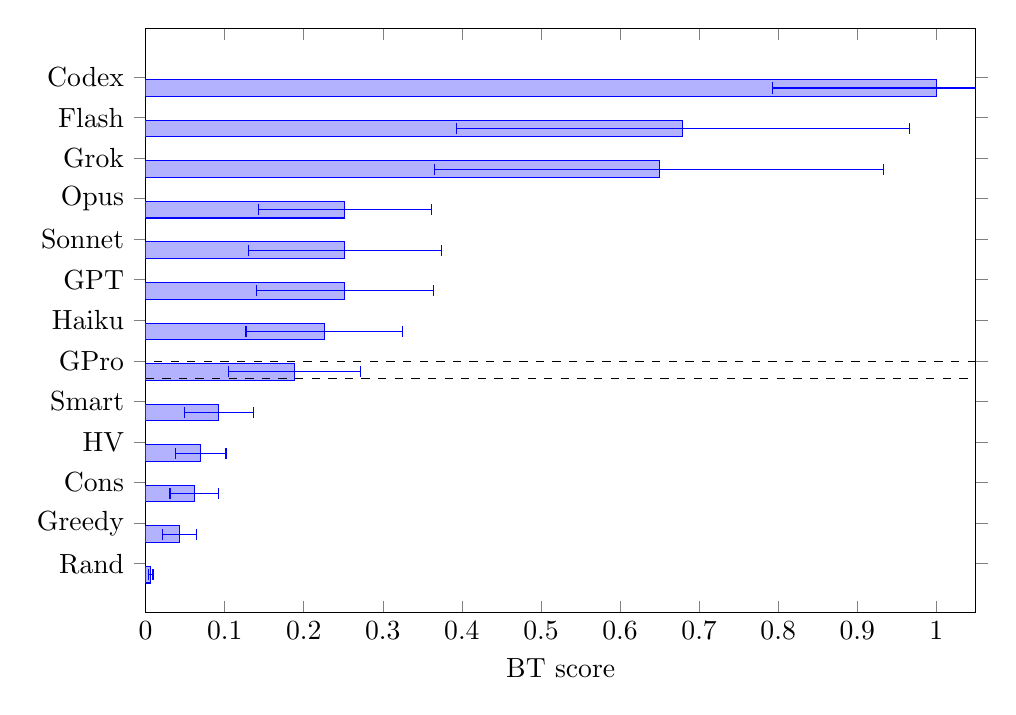
\begin{tikzpicture}
\begin{axis}[
xbar,
xmin=0, xmax=1.05,
height=9cm,
width=\columnwidth,
xlabel={BT score},
ytick={0,1,2,3,4,5,6,7,8,9,10,11,12},
yticklabels={Codex,Flash,Grok,Opus,Sonnet,GPT,Haiku,GPro,Smart,HV,Cons,Greedy,Rand},
y dir=reverse,
bar width=6pt,
error bars/x dir=both, error bars/x explicit,
]
\addplot+[error bars/x dir=both, error bars/x explicit] coordinates {
(1.0000,0) +- (0.2075,0.0000)
(0.6793,1) +- (0.2863,0.3207)
(0.6496,2) +- (0.2840,0.3504)
(0.2520,3) +- (0.1091,0.1414)
(0.2520,4) +- (0.1223,0.1746)
(0.2520,5) +- (0.1122,0.1697)
(0.2258,6) +- (0.0989,0.1334)
(0.1882,7) +- (0.0839,0.1226)
(0.0926,8) +- (0.0436,0.0539)
(0.0698,9) +- (0.0319,0.0383)
(0.0614,10) +- (0.0306,0.0415)
(0.0426,11) +- (0.0217,0.0335)
(0.0066,12) +- (0.0028,0.0035)
};
\addplot[black,dashed] coordinates {(0,7.5) (1.05,7.5)};
\end{axis}
\end{tikzpicture}
\caption{Tournament~002 BT scores with 95\% bootstrap CI. Dashed line separates LLMs (above) from baselines (below).}
\label{fig:t2_bt}
\end{figure}

\subsection{The new top tier: Codex, Flash, Grok}

\tTwo exhibits a clear top tier.
GPT-5.2-Codex ranks 1st (BT=1.000), Gemini Flash 2nd (BT=0.679), and Grok 3rd (BT=0.650).
There is a large gap from rank~3 to rank~4: BT drops from 0.650 to 0.252.
Pairwise, Grok beats Flash in 9/10 series (Table~\ref{tab:t2_matrix}) yet loses to Codex 2--8, illustrating the non-transitive dynamics that emerge under adaptation.

\subsection{Rank reshuffling across tournaments}

Table~\ref{tab:t1_t2_comp} and Figure~\ref{fig:rank_slope} summarize rank changes.
The \tTwo{} winner, GPT-5.2-Codex, achieves the largest BT gain ($+0.881$), jumping from rank~9 in \tOne{} to rank~1 in \tTwo.
Conversely, \tOne{} winner SmartAgent falls from rank~1 to rank~9 ($\Delta$BT=$-$0.907).
Claude Opus improves dramatically (BT 0.017$\to$0.252; a 14.6$\times$ increase) and ties for the largest rank jump ($+$8, shared with Codex), but remains the weakest Claude by Elo and still loses 0--10 to Claude Sonnet in both tournaments.

Three agents (Opus, Sonnet, GPT-5.2) share BT=0.252 in \tTwo; ordering among them is not statistically resolved.
We list them in the order returned by the BT fit and report Elo as an auxiliary metric.

\begin{table}[t]
\centering
\small
\caption{Tournament~001 vs Tournament~002 comparison. Positive $\Delta$Rank indicates improvement (lower rank number).}
\label{tab:t1_t2_comp}
\begin{tabular}{llrrrr}
\toprule
Agent & Type & R\textsubscript{T1} & R\textsubscript{T2} & $\Delta$R & $\Delta$BT \\
\midrule
GPT-5.2-Codex & LLM & 9 & 1 & +8 & +0.881 \\
Gemini Flash & LLM & 4 & 2 & +2 & +0.177 \\
Grok-4.1 Fast & LLM & 6 & 3 & +3 & +0.212 \\
Cl.\ Opus 4.6 & LLM & 12 & 4 & +8 & +0.235 \\
Cl.\ Sonnet 4.6 & LLM & 10 & 5 & +5 & +0.186 \\
GPT-5.2 & LLM & 8 & 6 & +2 & +0.022 \\
Cl.\ Haiku 4.5 & LLM & 11 & 7 & +4 & +0.169 \\
Gemini Pro & LLM & 5 & 8 & $-$3 & $-$0.267 \\
SmartAgent & Base & 1 & 9 & $-$8 & $-$0.907 \\
HighVariance & Base & 2 & 10 & $-$8 & $-$0.884 \\
Conservative & Base & 3 & 11 & $-$8 & $-$0.581 \\
Greedy & Base & 7 & 12 & $-$5 & $-$0.196 \\
Random & Base & 13 & 13 & 0 & +0.001 \\
\bottomrule
\end{tabular}
\end{table}

\begin{figure}[t]
\centering
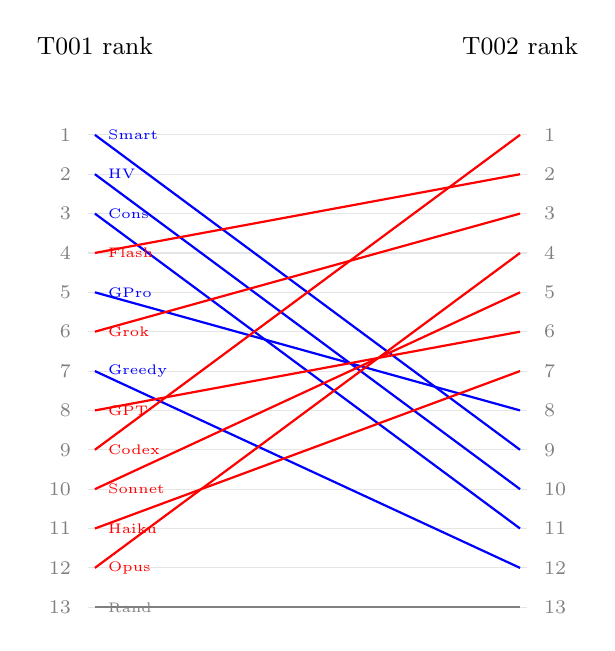
\begin{tikzpicture}[x=0.9cm,y=0.5cm]
\node[anchor=south,font=\small] at (0,0.8) {\tOne{} rank};
\node[anchor=south,font=\small] at (6,0.8) {\tTwo{} rank};
\foreach \i in {1,...,13} {
  \node[anchor=east,gray,font=\scriptsize] at (-0.2,-\i) {\i};
  \node[anchor=west,gray,font=\scriptsize] at (6.2,-\i) {\i};
  \draw[gray!20] (-0.1,-\i) -- (6.1,-\i);
}
\draw[thick,blue] (0,-1) -- (6,-9); \node[anchor=west,blue,font=\tiny] at (0.05,-1) {Smart};
\draw[thick,blue] (0,-2) -- (6,-10); \node[anchor=west,blue,font=\tiny] at (0.05,-2) {HV};
\draw[thick,blue] (0,-3) -- (6,-11); \node[anchor=west,blue,font=\tiny] at (0.05,-3) {Cons};
\draw[thick,red] (0,-4) -- (6,-2); \node[anchor=west,red,font=\tiny] at (0.05,-4) {Flash};
\draw[thick,blue] (0,-5) -- (6,-8); \node[anchor=west,blue,font=\tiny] at (0.05,-5) {GPro};
\draw[thick,red] (0,-6) -- (6,-3); \node[anchor=west,red,font=\tiny] at (0.05,-6) {Grok};
\draw[thick,blue] (0,-7) -- (6,-12); \node[anchor=west,blue,font=\tiny] at (0.05,-7) {Greedy};
\draw[thick,red] (0,-8) -- (6,-6); \node[anchor=west,red,font=\tiny] at (0.05,-8) {GPT};
\draw[thick,red] (0,-9) -- (6,-1); \node[anchor=west,red,font=\tiny] at (0.05,-9) {Codex};
\draw[thick,red] (0,-10) -- (6,-5); \node[anchor=west,red,font=\tiny] at (0.05,-10) {Sonnet};
\draw[thick,red] (0,-11) -- (6,-7); \node[anchor=west,red,font=\tiny] at (0.05,-11) {Haiku};
\draw[thick,red] (0,-12) -- (6,-4); \node[anchor=west,red,font=\tiny] at (0.05,-12) {Opus};
\draw[thick,gray] (0,-13) -- (6,-13); \node[anchor=west,gray,font=\tiny] at (0.05,-13) {Rand};
\end{tikzpicture}
\caption{Rank changes from \tOne{} to \tTwo{} (lower is better). Red: improved; blue: dropped; gray: unchanged.}
\label{fig:rank_slope}
\end{figure}

\subsection{Adaptation: when does feedback help?}

\tTwo{} allows the loser of each game to re-pick after seeing the winner's build.
Table~\ref{tab:t2_adapt} reports per-model adaptation propensity, build diversity, and post-loss outcomes conditional on adapting vs.\ sticking.

Across the eight LLMs, adaptation is common (1065 adaptations over 1591 losses; 66.9\%).
When an LLM agent changes its build after a loss, it wins 51.06\% of subsequent games; when it does not change, it wins 31.84\%.
However, adaptation rate is only weakly correlated with final BT (Spearman $\rho=0.19$ across LLMs), suggesting that finding strong builds early is often more important than reactive counter-picking.
Gemini Flash exemplifies this: it adapts in only 38\% of losses but achieves a 76\% win rate when it does, compared to 37\% when it sticks---it found strong builds fast and did not need to change often.

\begin{table}[t]
\centering
\footnotesize
\setlength{\tabcolsep}{3pt}
\caption{Tournament~002 adaptation metrics. ``Rate'' = $P[\text{adapt}\mid\text{lost}]$. SmartAgent re-evaluates via rollout; fixed-build baselines cannot adapt.}
\label{tab:t2_adapt}
\begin{tabular}{llrrrrll}
\toprule
Agent & BT & Blds & Lost & Adpt & Rate & Adpt WR & Stick WR \\
\midrule
Codex & 1.000 & 63 & 150 & 137 & 91\% & 61\% & 46\% \\
Flash & 0.679 & 17 & 151 & 58 & 38\% & 76\% & 37\% \\
Grok & 0.650 & 32 & 174 & 130 & 75\% & 64\% & 43\% \\
Opus & 0.252 & 6 & 219 & 116 & 53\% & 54\% & 31\% \\
Sonnet & 0.252 & 29 & 253 & 166 & 66\% & 63\% & 55\% \\
GPT & 0.252 & 45 & 211 & 188 & 89\% & 44\% & 35\% \\
Haiku & 0.226 & 32 & 232 & 191 & 82\% & 36\% & 46\% \\
GPro & 0.188 & 23 & 201 & 79 & 39\% & 35\% & 12\% \\
\midrule
Smart & 0.093 & 5 & 275 & 110 & 40\% & 39\% & 24\% \\
HV & 0.070 & 1 & 294 & 0 & 0\% & -- & 24\% \\
Cons & 0.061 & 1 & 286 & 0 & 0\% & -- & 21\% \\
Greedy & 0.043 & 1 & 292 & 0 & 0\% & -- & 21\% \\
Random & 0.007 & 1 & 360 & 0 & 0\% & -- & 0\% \\
\bottomrule
\end{tabular}
\end{table}

\subsection{Opus escapes the WIL trap---partially}

In \tOne, Claude Opus selects wolf builds exclusively with an average stat profile of 3.0/8.1/1.0/7.9 (HP/ATK/SPD/WIL) and achieves BT=0.017.
In \tTwo, Opus shifts toward high-ATK, low-WIL builds---primarily bear variants with avg stats 8.6/8.5/1.9/1.0---reaching BT=0.252 (a 14.6$\times$ improvement).
However, Opus remains brittle: it uses only 6 unique builds across all games (the fewest among LLMs), loses 0--10 to Sonnet, and loses 0--10 to Flash.
The WIL trap is broken by explicit formulas and meta context, but Opus's low build diversity suggests it converges too narrowly once it finds a viable strategy.

\subsection{Non-transitivity appears in \tTwo}

Unlike \tOne{} (0 strict 3-cycles), \tTwo{} contains 12 strict 3-cycles (triplets where $A>B$, $B>C$, $C>A$, all edges $>$50\%).
A representative cycle is: SmartAgent beats Sonnet (90\%), Sonnet beats Flash (60\%), and Flash beats SmartAgent (100\%).
The appearance of non-transitivity is consistent with adaptation creating genuine rock--paper--scissors dynamics: when agents can counter-pick, the meta is no longer a strict linear ordering.

\begin{table}[t]
\centering
\footnotesize
\setlength{\tabcolsep}{2.5pt}
\renewcommand{\arraystretch}{1.05}
\caption{Tournament~002 pairwise series win rates (\%, 10 series per matchup).}
\label{tab:t2_matrix}
\begin{tabular}{lrrrrrrrrrrrrr}
\toprule
 & Cx & Fl & Gr & Op & So & G5 & Ha & GP & Sm & HV & Co & Gy & Ra \\
\midrule
Cx & -- & 70 & 80 & 90 & 80 & 80 & 90 & 90 & 100 & 100 & 70 & 90 & 100 \\
Fl & 30 & -- & 10 & 100 & 40 & 80 & 100 & 100 & 100 & 100 & 100 & 100 & 100 \\
Gr & 20 & 90 & -- & 70 & 50 & 50 & 90 & 80 & 100 & 100 & 100 & 100 & 100 \\
Op & 10 & 0 & 30 & -- & 0 & 50 & 70 & 50 & 100 & 100 & 100 & 100 & 100 \\
So & 20 & 60 & 50 & 100 & -- & 50 & 60 & 70 & 10 & 90 & 60 & 40 & 100 \\
G5 & 20 & 20 & 50 & 50 & 50 & -- & 30 & 50 & 100 & 90 & 100 & 50 & 100 \\
Ha & 10 & 0 & 10 & 30 & 40 & 70 & -- & 90 & 60 & 70 & 100 & 100 & 100 \\
GP & 10 & 0 & 20 & 50 & 30 & 50 & 10 & -- & 70 & 90 & 100 & 100 & 100 \\
Sm & 0 & 0 & 0 & 0 & 90 & 0 & 40 & 30 & -- & 80 & 30 & 70 & 100 \\
HV & 0 & 0 & 0 & 0 & 10 & 10 & 30 & 10 & 20 & -- & 100 & 90 & 100 \\
Co & 30 & 0 & 0 & 0 & 40 & 0 & 0 & 0 & 70 & 0 & -- & 100 & 100 \\
Gy & 10 & 0 & 0 & 0 & 60 & 50 & 0 & 0 & 30 & 10 & 0 & -- & 100 \\
Ra & 0 & 0 & 0 & 0 & 0 & 0 & 0 & 0 & 0 & 0 & 0 & 0 & -- \\
\bottomrule
\end{tabular}
\vspace{0.3em}
\noindent\footnotesize{Column abbreviations as in Table~\ref{tab:t1_matrix}.}
\end{table}

\subsection{Build diversity vs.\ performance}

Figure~\ref{fig:diversity_scatter} overlays build diversity and BT for both tournaments.
In \tOne, baselines are strong despite fixed builds; among LLMs, exploration predicts performance ($\rho=0.81$).
In \tTwo, the relationship weakens: Codex wins with very high diversity (63 builds), while Flash wins with fast convergence (17 builds).
This suggests that under scaffolding, \emph{how} an agent explores matters more than \emph{how much}.

\begin{figure}[t]
\centering
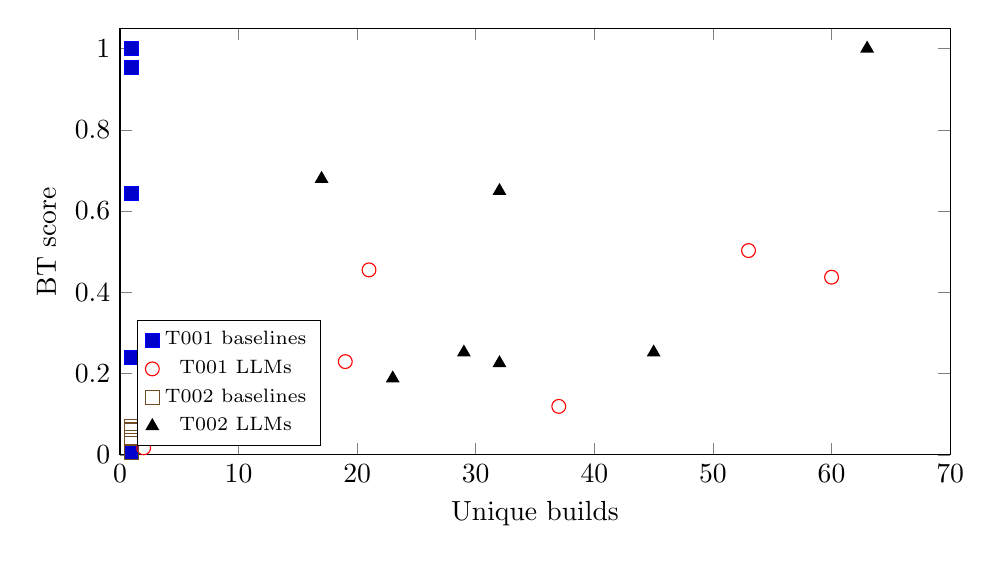
\begin{tikzpicture}
\begin{axis}[
width=\columnwidth, height=7cm,
xlabel={Unique builds},
ylabel={BT score},
xmin=0, xmax=70, ymin=0, ymax=1.05,
legend style={at={(0.02,0.02)},anchor=south west,font=\scriptsize},
]
\addplot+[only marks, mark=square*, mark size=2.5pt] coordinates {
(1,1.0000) (1,0.9541) (1,0.6426) (1,0.2388) (1,0.0054)
};
\addlegendentry{\tOne{} baselines}
\addplot+[only marks, mark=o, mark size=2.5pt] coordinates {
(53,0.5028) (21,0.4553) (60,0.4373) (19,0.2296) (37,0.1193) (3,0.0656) (9,0.0564) (2,0.0173)
};
\addlegendentry{\tOne{} LLMs}
\addplot+[only marks, mark=square, mark size=2.5pt] coordinates {
(5,0.0926) (1,0.0698) (1,0.0614) (1,0.0426) (1,0.0066)
};
\addlegendentry{\tTwo{} baselines}
\addplot+[only marks, mark=triangle*, mark size=2.5pt] coordinates {
(63,1.0000) (17,0.6793) (32,0.6496) (6,0.2520) (29,0.2520) (45,0.2520) (32,0.2258) (23,0.1882)
};
\addlegendentry{\tTwo{} LLMs}
\end{axis}
\end{tikzpicture}
\caption{Build diversity vs.\ BT score across both tournaments.}
\label{fig:diversity_scatter}
\end{figure}

\section{Tournament 003: Exact Rules + Feedback, No Meta}
\label{sec:t3}

Tournament~003 (\tThree) is a targeted ablation of \tTwo.
It preserves the same frozen simulator, exact mechanics, structured output, and loser-adapts protocol, but removes the meta-context block from the prompt.
The goal is to test whether the \tTwo{} reversal can be explained simply by models following the injected build hints, or whether some models remain strategically competent under exact mechanics and feedback alone.

\tThree{} contains 1050 completed best-of-7 series over 15 agents.
In addition to the original \tOne/\tTwo{} pool, we include two exploratory challengers: \texttt{gpt-5.3-codex} and \texttt{gpt-5.4}.
Prompt verification confirms that no build-hint block or meta-performance summary was present in the \tThree{} prompts.

\subsection{Meta removal splits the field rather than uniformly collapsing it}

Table~\ref{tab:t3_rank} and Figure~\ref{fig:t3_bt} show the primary \tThree{} ranking.
The key result is not a simple ``yes'' or ``no'' on whether meta context matters.
Instead, removing meta context \emph{splits the field}.

A subset of models remains strong with exact mechanics and feedback alone.
\texttt{gpt-5.2-codex} remains rank~1 (BT=1.000), \texttt{claude-opus-4-6} rises to rank~3 (BT=0.895), and \texttt{gpt-5.2} reaches rank~4 (BT=0.761).
These models therefore appear able to exploit the exact mechanics and the adaptation channel without needing explicit meta initialization.

By contrast, several models that were strong in \tTwo{} become brittle without meta hints.
\texttt{gemini-3-flash-preview}, \texttt{gemini-3.1-pro-preview}, and \texttt{grok-4-1-fast-reasoning} all collapse to the same single default build, use zero adaptation, and lose their top-tier status.
This reveals a model-specific dependence on meta initialization rather than a universal one.

\begin{table}[t]
\centering
\small
\caption{Tournament~003 rankings by Bradley--Terry score. \tThree{} is \tTwo{} minus meta-context.}
\label{tab:t3_rank}
\begin{tabular}{rll}
\toprule
Rank & Agent & BT (95\% CI) \\
\midrule
1 & \texttt{gpt-5.2-codex} & 1.0000 [0.615, 1.000] \\
2 & \texttt{SmartAgent} & 0.9839 [0.597, 1.000] \\
3 & \texttt{claude-opus-4-6} & 0.8952 [0.529, 1.000] \\
4 & \texttt{gpt-5.2} & 0.7607 [0.447, 1.000] \\
5 & \texttt{gemini-3.1-pro-preview} & 0.5461 [0.321, 0.731] \\
6 & \texttt{claude-sonnet-4-6} & 0.4650 [0.267, 0.628] \\
7 & \texttt{gemini-3-flash-preview} & 0.4511 [0.261, 0.586] \\
8 & \texttt{GreedyAgent} & 0.3741 [0.221, 0.493] \\
9 & \texttt{ConservativeAgent} & 0.3627 [0.212, 0.472] \\
10 & \texttt{grok-4-1-fast-reasoning} & 0.3532 [0.203, 0.466] \\
11 & \texttt{claude-haiku-4-5-20251001} & 0.3195 [0.187, 0.414] \\
12 & \texttt{HighVarianceAgent} & 0.2412 [0.134, 0.322] \\
13 & \texttt{gpt-5.3-codex} & 0.2345 [0.131, 0.316] \\
14 & \texttt{gpt-5.4} & 0.1750 [0.095, 0.231] \\
15 & \texttt{RandomAgent} & 0.0945 [0.049, 0.129] \\
\bottomrule
\end{tabular}
\end{table}

\begin{figure}[t]
\centering
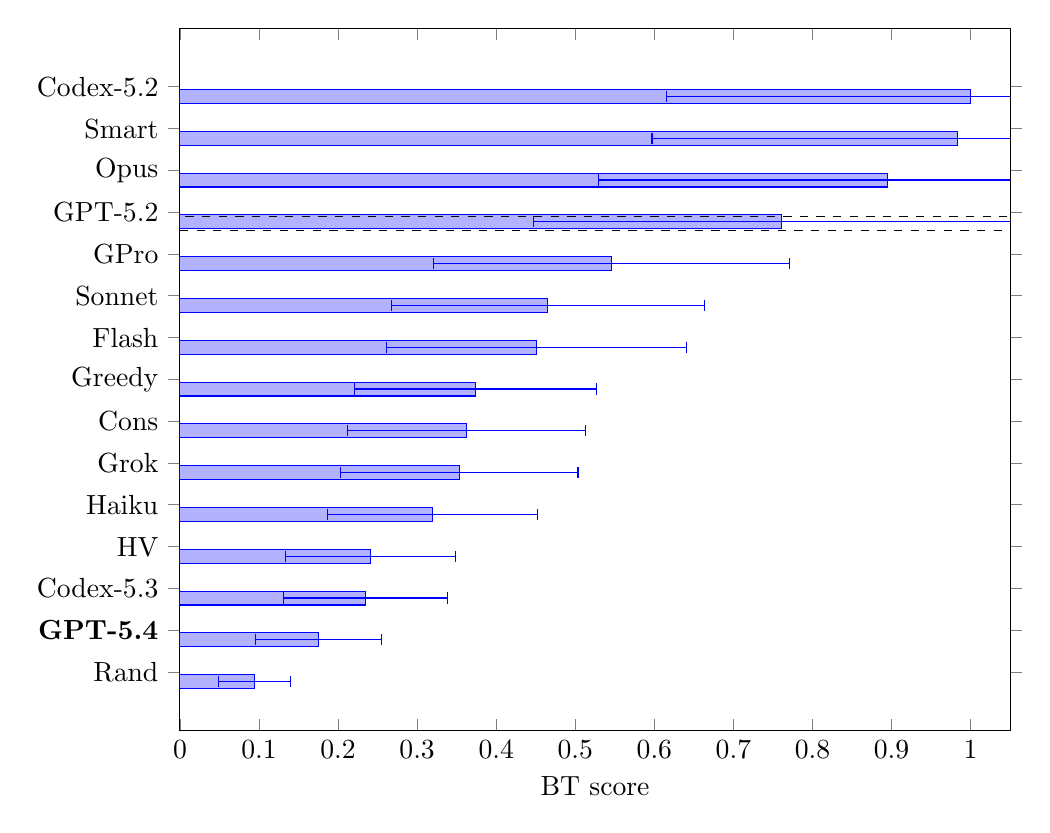
\begin{tikzpicture}
\begin{axis}[
xbar,
xmin=0, xmax=1.05,
height=10.5cm,
width=\columnwidth,
xlabel={BT score},
ytick={0,1,2,3,4,5,6,7,8,9,10,11,12,13,14},
yticklabels={Codex-5.2,Smart,Opus,GPT-5.2,GPro,Sonnet,Flash,Greedy,Cons,Grok,Haiku,HV,Codex-5.3,\textbf{GPT-5.4},Rand},
y dir=reverse,
bar width=5pt,
error bars/x dir=both, error bars/x explicit,
]
\addplot+[error bars/x dir=both, error bars/x explicit] coordinates {
(1.0000,0) +- (0.3850,0.0000)
(0.9839,1) +- (0.3869,0.0161)
(0.8952,2) +- (0.3662,0.1048)
(0.7607,3) +- (0.3137,0.2393)
(0.5461,4) +- (0.2251,0.1850)
(0.4650,5) +- (0.1980,0.1630)
(0.4511,6) +- (0.1901,0.1250)
(0.3741,7) +- (0.1531,0.1190)
(0.3627,8) +- (0.1507,0.1500)
(0.3532,9) +- (0.1502,0.1130)
(0.3195,10) +- (0.1325,0.0950)
(0.2412,11) +- (0.1072,0.0880)
(0.2345,12) +- (0.1035,0.0850)
(0.1750,13) +- (0.0800,0.0560)
(0.0945,14) +- (0.0455,0.0345)
};
\addplot[black,dashed] coordinates {(0,3.5) (1.05,3.5)};
\end{axis}
\end{tikzpicture}
\caption{Tournament~003 BT scores with 95\% bootstrap CI. Dashed line separates the meta-independent top tier (ranks 1--4) from the rest. GPT-5.4 (rank~14) is highlighted.}
\label{fig:t3_bt}
\end{figure}

\subsection{Robust search versus default-build collapse}

The clearest behavioral pattern in \tThree{} is not just ranking, but \emph{search behavior}.
Three models from three providers collapse to the exact same single build across the entire tournament:
\texttt{gemini-3-flash-preview}, \texttt{gemini-3.1-pro-preview}, and \texttt{grok-4-1-fast-reasoning} all play \texttt{BOAR 8/8/3/1} in 100\% of games and never adapt after losing.
The existence of exact mechanics and explicit loser adaptation is therefore not sufficient to guarantee active search.

By contrast, the strongest models remain exploratory.
\texttt{gpt-5.2-codex} uses 119 unique builds across 784 games, \texttt{gpt-5.2} uses 86 across 764 games, and \texttt{claude-opus-4-6} uses 12 across 762 games.
High performance does not require maximal diversity, but \tThree{} clearly distinguishes models that search from models that prematurely converge.

\begin{table}[t]
\centering
\footnotesize
\caption{Behavioral split in \tThree{} after removing meta-context. Dominant build share is the fraction of games played with the single most common build.}
\label{tab:t3_behavior}
\begin{tabular}{lrrrrr}
\toprule
Agent & BT & UB & Dom.\ build share & Post-loss adpt. & Rate \\
\midrule
\texttt{gpt-5.2-codex} & 1.000 & 119 & 6.6\% & 266 / 275 & 96.7\% \\
\texttt{claude-opus-4-6} & 0.895 & 12 & 46.6\% & 127 / 261 & 48.7\% \\
\texttt{gpt-5.2} & 0.761 & 86 & 13.5\% & 259 / 279 & 92.8\% \\
\midrule
\texttt{gemini-3-flash} & 0.451 & 1 & 100.0\% & 0 / 331 & 0.0\% \\
\texttt{gemini-3.1-pro} & 0.546 & 1 & 100.0\% & 0 / 310 & 0.0\% \\
\texttt{grok-4-1-fast} & 0.353 & 1 & 100.0\% & 0 / 328 & 0.0\% \\
\midrule
\texttt{gpt-5.4} & 0.175 & 79 & 11.4\% & 324 / 361 & 89.8\% \\
\bottomrule
\end{tabular}
\vspace{0.3em}
\noindent\footnotesize{UB = unique builds. Dom.\ = dominant.}
\end{table}

\subsection{Frontier capability does not automatically transfer to novel strategic domains}

\tThree{} provides a useful negative-transfer result.
\texttt{gpt-5.4}, a state-of-the-art frontier model released during this study, ranks 14th of 15 by BT, above only RandomAgent.
It finishes below all three fixed-strategy baselines (\texttt{GreedyAgent}, \texttt{ConservativeAgent}, and \texttt{HighVarianceAgent}) and far below the strongest adaptive models.

This result is notable not because it suggests the model is generally weak, but because it demonstrates that broad frontier capability---including strong performance on standard reasoning benchmarks, coding tasks, and professional knowledge work---does \emph{not} automatically transfer to a novel strategic domain.
Moreover, the failure is not caused by passivity: GPT-5.4 explores 79 unique builds and adapts after 89.8\% of losses, yet still performs poorly.
Search activity alone is insufficient; what matters is whether that search converges toward strategically strong regions of the build space.
This distinction between \emph{search volume} and \emph{search quality} is one of the clearest behavioral findings of \tThree.

\subsection{Meta-initialization dependence is heterogeneous, not universal}

The central scientific contribution of \tThree{} is that it rules out a reductive interpretation of \tTwo.
If the \tTwo{} performance reversal were driven solely by models following the injected top-build list, then removing meta context should cause all models to collapse together.
That does not happen.

\texttt{gpt-5.2-codex} remains rank~1 even with no build hints.
\texttt{claude-opus-4-6}, which failed catastrophically in \tOne, reaches rank~3 under exact mechanics plus feedback alone.
\texttt{gpt-5.2} remains in the top four.
These models therefore appear to possess a form of strategic competence that can operate without explicit meta initialization, provided the rules are exact and the feedback loop exists.

At the same time, other models appear strongly meta-dependent.
The simultaneous collapse of Flash, Pro, and Grok to the same single boar build suggests a different failure mode from the \tOne{} WIL trap:
not misunderstanding of the mechanics, but \emph{premature convergence to a reasonable-looking default when no external strategic anchor is provided}.
Thus, \tThree{} sharpens the interpretation of \tOne{} and \tTwo:
the critical moderator is not a uniform lack of strategic capability, but model-specific difficulty in initiating search without meta-level guidance.

\subsection{Non-transitivity persists under cleanroom conditions}

\tThree{} preserves the non-transitive character that emerged in \tTwo.
Using strict majority edges (win rate $>$50\%), we find 12 directed 3-cycles in the \tThree{} pairwise graph.
Importantly, these are not only baseline-vs-baseline effects.
There is also an all-LLM cycle:
\[
\texttt{claude-opus-4-6} > \texttt{gpt-5.2-codex} > \texttt{gpt-5.2} > \texttt{claude-opus-4-6},
\]
with series win rates 80\%, 60\%, and 60\%, respectively.
Thus, removing meta context does not collapse the game into a single total ordering.
What changes is not the presence of strategic richness, but which models can exploit it without hints.

\subsection{Prompt sensitivity validation}

A natural concern is whether the \tThree{} findings---particularly the field split and GPT-5.4's low ranking---are artifacts of the specific prompt wording rather than stable properties of the models.
To test this, we constructed a semantically equivalent paraphrase of the \tThree{} prompt (\texttt{t003\_v2.txt}) that preserves all exact formulas, the JSON output schema, and the loser-adapts mechanic while varying sentence structure and phrasing throughout.
We then ran a mini-tournament using five of the original agents: \texttt{claude-opus-4-6}, \texttt{claude-sonnet-4-6}, \texttt{gpt-5.4}, \texttt{SmartAgent}, and \texttt{GreedyAgent}.
(Gemini models were excluded due to API quota exhaustion; Grok was excluded due to persistent authentication failures.)

The resulting Bradley--Terry ranking under the paraphrased prompt reproduces the original \tThree{} ranking exactly:

\begin{table}[h]
\centering
\small
\caption{Prompt Sensitivity Index (PSI) validation: \tThree{} rankings under the original and a paraphrased prompt.}
\label{tab:psi}
\begin{tabular}{rlcc}
\toprule
Rank & Agent & Original BT & PSI BT \\
\midrule
1 & \texttt{SmartAgent} & 0.984 & 0.557 \\
2 & \texttt{claude-opus-4-6} & 0.895 & 0.195 \\
3 & \texttt{claude-sonnet-4-6} & 0.465 & 0.121 \\
4 & \texttt{GreedyAgent} & 0.374 & 0.102 \\
5 & \texttt{gpt-5.4} & 0.175 & 0.025 \\
\bottomrule
\end{tabular}
\end{table}

Kendall $\tau = 1.0$ (perfect rank correlation).
The absolute BT values differ between the two runs because fewer agents compress the scale, but the ordinal ranking is preserved without exception.
In particular, \texttt{gpt-5.4} remains last and LLMs collectively achieve only 37.7\% win rate against baselines---the same pattern observed in the full \tThree.

This result provides evidence that the \tThree{} findings---the field split, the default-build collapse of some models, and the negative-transfer result for GPT-5.4---are properties of the models' strategic reasoning rather than artifacts of a particular prompt surface form.
A full PSI suite across additional paraphrases and a broader agent set remains planned for future work.

\subsection{Caveats}

\tThree{} should be interpreted primarily as a causal ablation on \emph{LLM behavior}, not as a final baseline-vs-LLM leaderboard.
A remaining confound affects two baselines:
\texttt{RandomAgent} and \texttt{HighVarianceAgent} sample from the full 18-animal simulator enum, whereas the LLM prompt exposes only the six core animals.
This mismatch depresses these baselines in \tThree{} and weakens any blanket claim about baseline-vs-LLM ordering in the ablation.
The cleanest conclusions are therefore:
(i) meta-context is not uniformly required for strong play,
(ii) some models remain robust without it,
and (iii) others collapse into rigid default strategies when the meta anchor disappears.

\section{Discussion}

\paragraph{Comprehension vs.\ reasoning.}
The flip from \tOne{} to \tTwo{} implicates \emph{comprehension and representation} more than an absence of strategic capability.
In \tOne, LLMs must translate qualitative descriptions into an implicit quantitative model; baselines that encode numeric heuristics dominate.
In \tTwo, providing formulas and examples makes the same optimization problem tractable, and LLMs surpass baselines decisively.
The bottleneck in \tOne{} is not that LLMs ``cannot reason'' but that they cannot reliably extract quantitative structure from vague natural-language descriptions.

\paragraph{Feedback and adaptation.}
Within-series feedback is useful (Table~\ref{tab:t2_adapt}), but it is not the only path to success.
Codex adapts in 91\% of losses and wins with the highest build diversity.
Flash adapts in only 38\% of losses but achieves the highest per-adaptation win rate (76\%).
\tThree{} sharpens this picture further: access to adaptation does not imply that a model will actually \emph{use} adaptation as a search strategy.
Several \tThree{} models keep exact mechanics and feedback but never change their build after losing.
Thus, the benchmark now distinguishes between \emph{adaptation availability} and \emph{adaptation usage}.

\paragraph{Meta-initialization dependence.}
The meta block in \tTwo{} provides a strong initialization that \tOne{} lacks.
Notably, the injected meta context was itself imperfect: it was computed on a filtered subset of \tOne{} data, and all five builds showed 100\% win rate on small samples (4--22 games), somewhat overstating their true strength.
Despite this noise, the meta block was sufficient to shift the regime: LLM-vs-baseline series win rate increased from 37.50\% to 89.75\%.
\tThree{} shows that this effect is heterogeneous: some models remain strong with exact rules and feedback alone, whereas others depend heavily on the meta anchor.

\paragraph{Price--performance paradox.}
Across tournaments, Claude Opus is never the strongest Claude despite being the most expensive tier.
In \tOne, Sonnet is the strongest Claude by BT (0.066 vs.\ Opus's 0.017).
In \tTwo, Opus and Sonnet share BT=0.252 but Opus has the lowest Elo among Claude models (1526 vs.\ Sonnet's 1709 and Haiku's 1553).
In \tThree, Opus rebounds to rank~3, showing that its failures are highly prompt- and representation-sensitive rather than uniform.
Taken together, these results suggest that model cost and general helpfulness tuning do not imply robust strategic performance under Moreau.

\paragraph{Non-transitivity as a meta-complexity indicator.}
The appearance of 12 strict 3-cycles in both \tTwo{} and \tThree{} (vs.\ 0 in \tOne) suggests that exact mechanics plus adaptation create a richer strategic landscape.
Under one-shot play, the meta collapses toward ``stack ATK''; under adaptation, counter-picking and local search introduce genuine rock-paper-scissors structure.

\section{Limitations}
\label{sec:limits}

\begin{enumerate}[leftmargin=*]
\item \textbf{Multiple simultaneous interventions in \tTwo.}
\tTwo{} introduces four major changes at once (exact formulas, meta context, per-game adaptation with winner lock, structured output schema), so we cannot attribute the performance reversal to any single factor.
\tThree{} isolates one component (meta context); further ablations are needed to disentangle the remaining three.

\item \textbf{Prompt dependence is part of the construct.}
The large \tOne$\to$\tTwo swing highlights that ``strategy'' and ``prompt engineering'' interact tightly.
This is a feature, not a bug: Moreau Arena intentionally stresses rule comprehension, and the prompt sensitivity itself is a measurable result.
An initial prompt sensitivity analysis on \tThree{} yields Kendall $\tau=1.0$ (Table~\ref{tab:psi}), indicating perfect rank preservation under one paraphrase.
However, this validation covers a single paraphrase and a subset of agents (5 of 15); a broader prompt sensitivity suite across the full agent pool remains needed.

\item \textbf{Statistical resolution.}
Each pair plays 10 series.
Confidence intervals overlap for several adjacent LLM ranks (Tables~\ref{tab:t1_rank}--\ref{tab:t3_rank}); finer-grained ordering would benefit from more series.
Three agents share BT=0.252 in \tTwo, and their relative ordering is not statistically resolved.

\item \textbf{Decoding settings.}
Temperature and sampling differ across provider defaults and were not swept.
A controlled decoding ablation may change relative performance among closely ranked LLMs.

\item \textbf{No human baseline.}
We do not yet include human players, which would provide a useful anchor for interpreting LLM performance.

\item \textbf{Meta context fidelity.}
The \tTwo{} meta block was extracted from a filtered subset of \tOne{} data (excluding floor baselines), yielding uniformly 100\% win rates on small samples.
The injected builds are strong but their stated win rates overestimate true population rates.
We document the exact injected text in Appendix~\ref{app:t2_prompt}.

\item \textbf{Baseline-pool mismatch in \tThree.}
In \tThree{}, two baselines (\texttt{RandomAgent} and \texttt{HighVarianceAgent}) operate over the full simulator roster, while prompt-visible LLM actions are restricted to the six core animals.
This weakens baseline-vs-LLM comparisons in \tThree{} and motivates a controlled rerun under a matched action space in future work.
\end{enumerate}

\section{Future Work}
\label{sec:future}

The most important next step is a series of ablations to isolate each remaining \tTwo{} intervention:
(a) exact formulas only (no meta, no adaptation);
(b) meta context only (no adaptation);
(c) adaptation only (vague prompt).
These ablations will support causal rather than correlational claims about which scaffolding component drives the performance reversal.

We plan to formalize Moreau Arena as a \emph{tiered measurement battery} with standardized tracks:
Track~A (one-shot, as in \tOne),
Track~B (feedback adaptation, as in \tTwo),
Track~C (exact rules + feedback without meta, as in \tThree),
and Track~D (tool-augmented, where agents may use a calculator or limited simulator).
Each track measures a distinct axis of strategic competence; results should not be compared across tracks.

Additional planned extensions include:
enabling the auto-balancer between tournaments to study non-stationary metas;
adding human baselines (competitive gamers given the same prompt and time budget);
analyzing reasoning traces to understand \emph{why} some models explore more broadly;
running an expanded prompt sensitivity suite (additional paraphrases across the full 15-agent pool, including models excluded from the initial validation due to API limitations) and reporting rank stability across prompt variants;
and a controlled \tThree{} rerun with baselines restricted to the same six prompt-visible animals.

\section{Ethics and Responsible Benchmarking}

Moreau Arena is designed to support responsible benchmarking:
(i) a newly authored ruleset to reduce contamination risk,
(ii) deterministic execution under hashed seeds (the simulator is deterministic given the recorded actions and the seed; LLM sampling may be stochastic, so reproducibility is achieved by recording actions, decoding settings, and seeds),
(iii) a frozen configuration snapshot for reproducibility,
and (iv) a planned auto-balancing mechanism to mitigate overfitting to a static meta in long-running leaderboards.
We present results as descriptive measurements of capability and failure mode, avoiding normative claims about intent or deception.
Strong performance under heavy scaffolding (\tTwo) or partial robustness under no-meta conditions (\tThree) does not imply robust decision-making in safety-critical domains; we recommend reporting results under multiple prompt regimes.

\section{Conclusion}

Three tournaments over a shared Moreau Arena core reveal a sharp boundary condition for LLM strategic reasoning.
Under a vague, one-shot prompt with no feedback (\tOne, 779 series), handcrafted baselines dominate and LLMs exhibit qualitative traps---most notably the WIL trap, where compositional failure (large-looking percentages modulating rare events) leads to systematically dominated builds.
When mechanics are explicit, examples are provided, and feedback is allowed (\tTwo, 780 series), the leaderboard reverses completely: every LLM outranks every baseline.
When the same exact mechanics and feedback remain but meta context is removed (\tThree, 1050 series), the field splits: some models remain strong without hints, while others collapse to rigid default builds and stop adapting.

The most important result is the gap structure itself.
It suggests that for strategic tasks, the limiting factor is often not the existence of reasoning machinery but whether the task representation and feedback channel allow that machinery to operate---and whether the model can initiate search without an explicit strategic anchor.
GPT-5.2-Codex's path is the clearest example: near-bottom in \tOne, first in \tTwo, and still first in \tThree.
At the same time, GPT-5.4's weak \tThree{} result shows that frontier capability does not automatically transfer to novel strategic domains: active search without convergence toward strong builds produces worse outcomes than a fixed heuristic.
An initial prompt sensitivity analysis (Kendall $\tau=1.0$ under a semantically equivalent paraphrase) confirms that these findings are properties of the models, not artifacts of prompt wording.

We release the complete prompts, configuration hashes, match records, and analysis code at \url{https://moreauarena.com} to support reproducibility and follow-up studies.

\section*{Use of Generative AI Tools (Disclosure)}
Generative AI language tools were used (i) as \emph{subjects} in the tournament experiments analyzed; and (ii) as writing aids for drafting and editing.
No AI system is listed as an author.
All claims, data verification, interpretations, and final wording were selected and reviewed by the human author, who takes responsibility for the content and any remaining errors.

\section*{Acknowledgements}
I thank collaborators in the Round Table research group for methodological discussions, and the AI models (Claude, Gemini, Grok) that served as both experimental subjects and research tools throughout this project, and the model providers whose APIs made the experiments possible.
Any errors or misinterpretations are my own.

\begin{thebibliography}{99}

\bibitem{bradley_terry}
R.~A.~Bradley and M.~E.~Terry.
\newblock Rank analysis of incomplete block designs: {I}. {T}he method of paired comparisons.
\newblock \emph{Biometrika}, 39(3/4):324--345, 1952.

\bibitem{pluribus}
N.~Brown and T.~Sandholm.
\newblock Superhuman {AI} for multiplayer poker.
\newblock \emph{Science}, 365(6456):885--890, 2019.

\bibitem{cicero}
A.~Bakhtin et~al.
\newblock Human-level play in the game of {D}iplomacy by combining language models with strategic reasoning.
\newblock \emph{Science}, 378(6624):1067--1074, 2022.

\bibitem{nle}
H.~K{\"u}ttler et~al.
\newblock The {N}et{H}ack {L}earning {E}nvironment.
\newblock In \emph{NeurIPS}, 2020.

\bibitem{procgen}
K.~Cobbe et~al.
\newblock Leveraging procedural generation to benchmark reinforcement learning.
\newblock In \emph{ICML}, 2020.

\bibitem{min2022}
S.~Min et~al.
\newblock Rethinking the role of demonstrations: What makes in-context learning work?
\newblock In \emph{EMNLP}, 2022.

\bibitem{wei2022}
J.~Wei et~al.
\newblock Chain-of-thought prompting elicits reasoning in large language models.
\newblock In \emph{NeurIPS}, 2022.

\bibitem{helm}
P.~Liang et~al.
\newblock Holistic evaluation of language models.
\newblock \emph{arXiv preprint arXiv:2211.09110}, 2022.

\bibitem{chatbot_arena}
L.~Zheng et~al.
\newblock Judging {LLM}-as-a-judge with {MT}-{B}ench and {C}hatbot {A}rena.
\newblock \emph{arXiv preprint arXiv:2306.05685}, 2023.

\bibitem{mmlu}
D.~Hendrycks et~al.
\newblock Measuring massive multitask language understanding.
\newblock In \emph{ICLR}, 2021.

\bibitem{gsm8k}
K.~Cobbe et~al.
\newblock Training verifiers to solve math word problems.
\newblock \emph{arXiv preprint arXiv:2110.14168}, 2021.

\bibitem{arc}
F.~Chollet.
\newblock On the measure of intelligence.
\newblock \emph{arXiv preprint arXiv:1911.01547}, 2019.

\bibitem{bigbench}
A.~Srivastava et~al.
\newblock Beyond the imitation game: Quantifying and extrapolating the capabilities of language models.
\newblock \emph{arXiv preprint arXiv:2206.04615}, 2022.

\bibitem{orak}
KRAFTON AI.
\newblock Orak: A Multi-Game Benchmark for LLM Agents.
\newblock In \emph{ICLR}, 2026.

\end{thebibliography}

\appendix

\section{Tournament~001 prompt}\label{app:t1_prompt}

The following reproduces the prompt shown to every LLM in Tournament~001 (from \texttt{build\_prompt(opponent\_animal=None, banned=[])} in \texttt{src/moreau/llm\_agent.py}; line breaks adjusted only for page width).

\begingroup
\small
\begin{verbatim}
You are designing a creature for Moreau Arena,
a 1v1 combat game on an 8x8 grid.

RULES:
- Allocate exactly 20 stat points across 4 stats:
  HP, ATK, SPD, WIL (each minimum 1)
- Stat formulas:
    max_hp = 50 + 10 * HP
    base_dmg = floor(2 + 0.85 * ATK)
    dodge = SPD * 2.5%  (capped 30%)
    resist = min(60%, WIL * 3.3%)
- Closing Ring starts at tick 30, dealing increasing
  damage to creatures on outer tiles
- Abilities proc randomly each tick based on
  proc chance

AVAILABLE ANIMALS:
  BEAR - Passive: Fury Protocol - gains +ATK
    when damaged
    Abilities: Berserker Rage: +ATK buff for
    3 ticks (3.5% proc); Last Stand: 2x damage
    when below 15% HP (single charge, 3.5% proc)
  BUFFALO - Passive: Thick Hide - takes reduced
    damage
    Abilities: Thick Hide: Reduces incoming damage
    for 1 tick (4.5% proc); Iron Will: Survives
    a killing blow at 1 HP (single charge, 3.5%
    proc)
  BOAR - Passive: Charge - bonus damage on
    first hit
    Abilities: Stampede: AoE damage + knockback
    (4.5% proc); Gore: 0.6x damage but ignores
    dodge (3.5% proc)
  TIGER - Passive: Ambush Wiring - high dodge,
    first-strike advantage
    Abilities: Pounce: +70% damage + stun (4.5%
    proc); Hamstring: -55% SPD, -10% dodge for
    4 ticks (4.5% proc)
  WOLF - Passive: Pack Sense - bonus to ability
    proc chance
    Abilities: Pack Howl: +ATK buff for 4 ticks
    (4.5% proc); Rend: DoT bleed for 3 ticks
    (4.5% proc)
  MONKEY - Passive: Primate Cortex - adaptive,
    copies opponent abilities
    Abilities: Chaos Strike: Random damage
    multiplier 0.5x-2.0x (4.5% proc); Mimic:
    Copies opponent's last ability (3.5% proc)

Choose an animal and allocate 20 stat points.
Respond ONLY in this exact format:
ANIMAL HP ATK SPD WIL
Example: BOAR 8 8 3 1
\end{verbatim}
\endgroup

\noindent All LLM calls used \texttt{max\_tokens=64} with a 120-second hard timeout.
Invalid outputs triggered one retry; persistent failures fell back to GreedyAgent (\texttt{boar 8/8/3/1}).

\section{Tournament~002 prompt additions}\label{app:t2_prompt}

\tTwo{} augments the \tOne{} prompt with three blocks: (1) explicit numerical formulas for all passives and abilities, (2) metagame context automatically extracted from \tOne{} match records, and (3) a JSON output schema enforced via provider-specific structured output APIs.

\paragraph{Exact numerical formulas (excerpt).}
\begingroup
\small
\begin{verbatim}
STAT FORMULAS:
  max_hp = 50 + 10 * HP
  base_dmg = floor(2 + 0.85 * ATK)
  dodge_chance = min(30%, SPD * 2.5%)
  ability_resist = min(60%, WIL * 3.3%)
  ability_proc_bonus = WIL * 0.08% (additive)

PASSIVE DETAILS:
  BEAR - Fury Protocol: +1 ATK per hit taken
    (permanent, stacks)
  BUFFALO - Thick Hide: incoming damage
    reduced by 15%
  BOAR - Charge: first attack deals 1.5x damage
  TIGER - Ambush Wiring: +10% base dodge,
    attacks first on tick 1
  WOLF - Pack Sense: +1.5% additive to all
    ability proc rates
  MONKEY - Primate Cortex: 20% chance to copy
    opponent's last proc
\end{verbatim}
\endgroup

\paragraph{Meta context (exact text injected into every \tTwo{} prompt).}
The following was generated automatically by \texttt{meta\_extractor.py}, which filters out floor baselines (RandomAgent, HighVarianceAgent) and ranks remaining builds by win rate on the filtered subset.
All five builds show 100\% win rate on their respective subsamples; game-level win rates across all agents are lower (80--100\%).

\begingroup
\small
\begin{verbatim}
META CONTEXT (top builds from previous tournament,
ranked by win rate):
  1. BEAR 8/8/3/1  - 100% win rate (22 games)
  2. BEAR 8/10/1/1 - 100% win rate (19 games)
  3. BEAR 10/8/1/1 - 100% win rate (11 games)
  4. WOLF 7/10/2/1 - 100% win rate (4 games)
  5. BEAR 9/9/1/1  - 100% win rate (4 games)
\end{verbatim}
\endgroup

\paragraph{JSON output schema.}
\begingroup
\small
\begin{verbatim}
Respond ONLY with valid JSON:
{"animal":"BEAR","hp":3,"atk":14,"spd":2,"wil":1}

Rules: animal in {BEAR,BUFFALO,BOAR,TIGER,WOLF,
MONKEY}, hp+atk+spd+wil=20, each stat >= 1.
\end{verbatim}
\endgroup

\noindent Structured output was enforced via provider-specific APIs (Anthropic \texttt{tool\_use}, OpenAI \texttt{json\_schema}, Google \texttt{response\_schema}, xAI JSON mode).
Regex fallback was available but triggered zero times across all 780 \tTwo{} series.

\section{Tournament~003 prompt note}\label{app:t3_prompt}

Tournament~003 is identical to Tournament~002 except that the \texttt{META CONTEXT} block shown in Appendix~\ref{app:t2_prompt} is omitted entirely.
Exact formulas, structured JSON outputs, and loser adaptation remain enabled.

\end{document}
